\chapter{Testování vyvinutého řešení}
Testování a vývoj algoritmu byl prováděn především empiricky. K dispozici byl nejdříve malý vzorek dat, který byl dodán Fakultní nemocnicí Hradec Králové. Tento vzorek obsahoval 21 patologických videí, kde se vyskytovaly různé nemoci a 16 videí bez patologických výskytů. Každý snímek obsahoval 201 framů. Jelikož tato data byla extrahována za pomocí proprietárního softwaru dodávaného ke kamerám, tak kvalita dat nebyla nijak valná. U toho vzorku bylo lékaři označeno i, to co je na snímkách špatně.

Druhý vzorek dat byl získán od nemocnice až po vyvinutí algoritmů a softwaru. Měl tedy za úkol prokázat vyvinuté řešení na větším vzorku dat. U toho vzorku se však postrádá informace od profesionálů, jaká část obsahuje patologické nálezy a kvůli velkému množství dat to lze určit jen přibližně. Celkem se jedná o tři celé průchody kamerou, kde je patologický nález. Dva průchodu jsou z kamery PillCam celkem o 23608 framech a zbývající je z kamery od výrobce EndoCapsule o 87076 framech. Tento soubor dat je výrazně kvalitnější, jelikož ve spolupráci s akademií věd České republiky bylo použito jejich technologií pro extrakci dat z kamer. Na obrázku \ref{fig:vzorky} je vidět rozdíl v kvalitě obou vzorků.

\begin{figure}[h]
	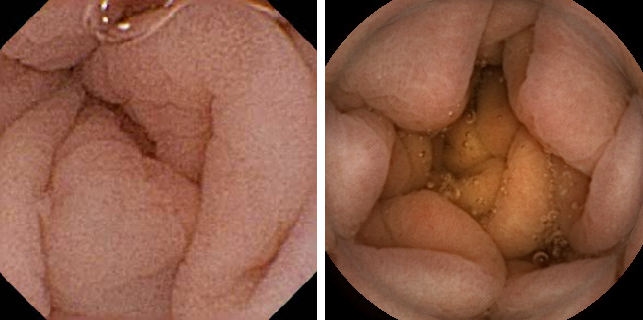
\includegraphics[scale=0.5]{vzorky}
	\centering
	\caption{Ukázka rozdílů kvality obou vzorků. Vlevo první vzorek, vpravo druhý vzorek \label{fig:vzorky}}
\end{figure} 

Vývoj a testování algoritmu detekce malých skvrn probíhal v různých etapách a od původního návrhu algoritmu do dnešní podoby se změnilo hodně věcí a byly použity jiné přístupy. Původní návrh byl nejdříve založen na adaptivním binárním práhování, ale to bylo zcela neúspěšné. Později byla snaha detekovat krvavé skvrny pomocí hranových detektorů konkrétně Cannyho detektor. To vedlo k lepšímu výsledku, nicméně chybovost byla příliš veliká a hrany se občas ztráceli vůči pozadí. Nakonec bylo zvoleno filtrování barev v HSV spektru, kde bylo dosaženo nejlepších výsledků a v kombinaci s hranovým detektorem pro odstranění míst bez hran se jeví jako optimální řešení. Testování později odhalilo, zejména v druhém vzorku dat, že druhý filtr barev pro zpřesnění výsledků není tak důležitý a jeho dopad v konečném výsledku není příliš markantní.

Druhý algoritmus byl značně přímočařejší a vzhledem k tomu, že autor již měl zkušenosti z prvního algoritmu, tak se spíše jednalo o nastavování správných hodnot v konfiguraci.

\section{Metodologie testování}
\label{sec:metodologie}
Pro měření úspěšnosti algoritmů jsou použity standardní postupy v počítačovém vidění pro určení efektivity algoritmu. Je tedy vypočítána hodnota \gls{glos:FRR} a \gls{glos:FAR} dle následujících vzorců.
\begin{equation*}
\gls{glos:FRR} = \frac{\gls{glos:FN}}{\gls{glos:TP}+\gls{glos:TN}+\gls{glos:FP}+\gls{glos:FN}} 
\end{equation*}
\begin{equation*}
\gls{glos:FAR} = \frac{\gls{glos:FP}}{\gls{glos:TP}+\gls{glos:TN}+\gls{glos:FP}+\gls{glos:FN}} 
\end{equation*}
V klinických testech se v lékařské komunitě používají hodnoty Senzitivita (\gls{glos:SE}) a Specificita (\gls{glos:SP})\cite{clinical}. Senzitivita je procentuální šance na detekci pacienta, který je nemocný a není tak špatně označen jako zdravý. Dalo by se říct, že opakem senzitivity je specificita. Při specificitě se jedná o správné detekování pacienta, který není nemocný a není špatně označen, jako pozitivní. Určuje se dle následujících vzorců.
\begin{equation*}
\gls{glos:SE} = \frac{\gls{glos:TP}}{\gls{glos:TP}+\gls{glos:FN}} 
\end{equation*}
\begin{equation*}
\gls{glos:SP} = \frac{\gls{glos:TN}}{\gls{glos:TN}+\gls{glos:FP}} 
\end{equation*}

V tabulce \ref{tab:vzorky} je vidět, kolik je skutečně pozitivních snímků v každém vzorku. Do tabulky jsou zahrnuty pouze ty vzorky, které obsahují krev. Ostatní vzorky buď obsahují jiné nemoci, nebo nejsou pozitivní. Každý vzorek také vždy neobsahuje krev, jež se dá snadno detekovat. Např. na vzorku z endocapsule je po cca 50\% vzorku masivní krvácení, kde se pak na každém snímku od vzniku problému vyskytuje alespoň slabá, místy růžová krev, která je již smíchána s jinými tekutinami, a tak nevyznačuje známky krve definované v algoritmu (dalo by se říct, že často je to spíše růžová voda). Počet snímků s krví u všech případů není úplně přesný, protože autor nemá k dispozici přesné počty, a tak musel vzorky projít ručně a provést odhad, který může být lehce nepřesný.

\begin{table}[h]
	\centering
	\begin{tabular}{|c|c|c|}
		\hline
		\bf Název souboru &  \bf Počet snímků & \bf Počet snímků s krví \\ \hline
		Endocapsule & 87076 & 45320 \\ \hline
		PillCam 1 & 13433 & 32 \\ \hline
		PillCam 2 & 10175 & 15 \\ \hline
		PAT07.avi & 201 & 5 \\ \hline
	\end{tabular}
	\caption{Jednotlivé vzorky s počtem krvavých snímků}
	\label{tab:vzorky}
\end{table}
\section{Výsledky testování}
Následující tabulka \ref{tab:vyslekdy_1} a \ref{tab:vyslekdy_2} ukazuje výsledky testování. Byly testovány všechny vzorky, vždy dle konfigurace pro ně určené. Pro jaký vzorek byla která konfigurace použita, je vidět v příloze \ref{sec:prilohaKonfig}. Ve výsledkových tabulkách jsou brány oba algoritmy jako jeden, a to z toho důvodu, že pro určení konečného výsledku je irelevantní, jestli to detekoval algoritmus A nebo B. Proto jsou vzaty výsledky obou algoritmů a je provedeno sjednocení. Také by bylo velmi problematické určit, co který algoritmus má detekovat a podle toho ho také hodnotit. Vybrané konkrétní výsledky algoritmů jsou vidět na obrázku \ref{fig:vysledy}. 
\begin{table}[h]
	\begin{adjustwidth}{-.5in}{-.5in} 
	\centering
	\begin{tabular}{|c|c|c|c|c|c|c|c|c|c|}
		\hline
		\bf Název souboru & \bf Detekováno & \bf \gls{glos:TP} & \bf \gls{glos:FP} & \bf \gls{glos:TN} & \bf \gls{glos:FN} & \bf \gls{glos:FRR} & \bf \gls{glos:FAR} & \bf \gls{glos:SE} & \bf \gls{glos:SP} \\ \hline
		PAT21.avi & 0 & 0 & 0 & 201 & 0 & 0,00\% & 0,00\% & N/A & 100,00\% \\ \hline
		PAT20.avi & 0 & 0 & 0 & 201 & 0 & 0,00\% & 0,00\% & N/A & 100,00\% \\ \hline
		PAT19.avi & 0 & 0 & 0 & 201 & 0 & 0,00\% & 0,00\% & N/A & 100,00\% \\ \hline
		PAT18.avi & 0 & 0 & 0 & 201 & 0 & 0,00\% & 0,00\% & N/A & 100,00\% \\ \hline
		PAT17.avi & 1 & 0 & 1 & 200 & 0 & 0,00\% & 0,50\% & N/A & 99,50\% \\ \hline
		PAT16.avi & 5 & 0 & 5 & 196 & 0 & 0,00\% & 2,49\% & N/A & 97,51\% \\ \hline
		PAT15.avi & 1 & 0 & 1 & 200 & 0 & 0,00\% & 0,50\% & N/A & 99,50\% \\ \hline
		PAT14.avi & 1 & 0 & 1 & 200 & 0 & 0,00\% & 0,50\% & N/A & 99,50\% \\ \hline
		PAT13.avi & 0 & 0 & 0 & 201 & 0 & 0,00\% & 0,00\% & N/A & 100,00\% \\ \hline
		PAT12.avi & 0 & 0 & 0 & 201 & 0 & 0,00\% & 0,00\% & N/A & 100,00\% \\ \hline
		PAT11.avi & 0 & 0 & 0 & 201 & 0 & 0,00\% & 0,00\% & N/A & 100,00\% \\ \hline
		PAT10.avi & 0 & 0 & 0 & 201 & 0 & 0,00\% & 0,00\% & N/A & 100,00\% \\ \hline
		PAT09.avi & 0 & 0 & 0 & 201 & 0 & 0,00\% & 0,00\% & N/A & 100,00\% \\ \hline
		PAT08.avi & 0 & 0 & 0 & 201 & 0 & 0,00\% & 0,00\% & N/A & 100,00\% \\ \hline
		PAT07.avi & 4 & 4 & 0 & 196 & 1 & 0,50\% & 0,00\% & 80,00\% & 100,00\% \\ \hline
		PAT06.avi & 0 & 0 & 0 & 201 & 0 & 0,00\% & 0,00\% & N/A & 100,00\% \\ \hline
		PAT05.avi & 0 & 0 & 0 & 201 & 0 & 0,00\% & 0,00\% & N/A & 100,00\% \\ \hline
		PAT04.avi & 0 & 0 & 0 & 201 & 0 & 0,00\% & 0,00\% & N/A & 100,00\% \\ \hline
		PAT03.avi & 0 & 0 & 0 & 201 & 0 & 0,00\% & 0,00\% & N/A & 100,00\% \\ \hline
		PAT02.avi & 3 & 0 & 3 & 198 & 0 & 0,00\% & 1,49\% & N/A & 98,51\% \\ \hline
		PAT01.avi & 0 & 0 & 0 & 201 & 0 & 0,00\% & 0,00\% & N/A & 100,00\% \\ \hline
		NOR9.avi & 0 & 0 & 0 & 201 & 0 & 0,00\% & 0,00\% & N/A & 100,00\% \\ \hline
		NOR8.avi & 0 & 0 & 0 & 201 & 0 & 0,00\% & 0,00\% & N/A & 100,00\% \\ \hline
		NOR7.avi & 2 & 0 & 2 & 199 & 0 & 0,00\% & 1,00\% & N/A & 99,00\% \\ \hline
		NOR6.avi & 0 & 0 & 0 & 201 & 0 & 0,00\% & 0,00\% & N/A & 100,00\% \\ \hline
		NOR5.avi & 0 & 0 & 0 & 201 & 0 & 0,00\% & 0,00\% & N/A & 100,00\% \\ \hline
		NOR4.avi & 0 & 0 & 0 & 201 & 0 & 0,00\% & 0,00\% & N/A & 100,00\% \\ \hline
		NOR3.avi & 0 & 0 & 0 & 201 & 0 & 0,00\% & 0,00\% & N/A & 100,00\% \\ \hline
		NOR2.avi & 0 & 0 & 0 & 201 & 0 & 0,00\% & 0,00\% & N/A & 100,00\% \\ \hline
		NOR16.avi & 0 & 0 & 0 & 201 & 0 & 0,00\% & 0,00\% & N/A & 100,00\% \\ \hline
		NOR15.avi & 0 & 0 & 0 & 201 & 0 & 0,00\% & 0,00\% & N/A & 100,00\% \\ \hline
		NOR14.avi & 0 & 0 & 0 & 201 & 0 & 0,00\% & 0,00\% & N/A & 100,00\% \\ \hline
		NOR13.avi & 0 & 0 & 0 & 201 & 0 & 0,00\% & 0,00\% & N/A & 100,00\% \\ \hline
		NOR12.avi & 0 & 0 & 0 & 201 & 0 & 0,00\% & 0,00\% & N/A & 100,00\% \\ \hline
		NOR11.avi & 0 & 0 & 0 & 201 & 0 & 0,00\% & 0,00\% & N/A & 100,00\% \\ \hline
		NOR10.avi & 0 & 0 & 0 & 201 & 0 & 0,00\% & 0,00\% & N/A & 100,00\% \\ \hline
		NOR1.avi & 47 & 0 & 47 & 154 & 0 & 0,00\% & 23,38\% & N/A & 76,62\% \\ \hline
	\end{tabular}
	\caption{Výsledky testování prvního vzorku}
	\label{tab:vyslekdy_1}
	\end{adjustwidth}
\end{table}

\begin{table}[h]
	\begin{adjustwidth}{-.5in}{-.5in} 
		\centering
		\begin{tabular}{|c|c|c|c|c|c|c|c|c|c|}
			\hline
				\bf Název souboru & \bf Detekováno & \bf \gls{glos:TP} & \bf \gls{glos:FP} & \bf \gls{glos:TN} & \bf \gls{glos:FN} & \bf \gls{glos:FRR} & \bf \gls{glos:FAR} & \bf \gls{glos:SE} & \bf \gls{glos:SP} \\ \hline
			Endocapsule & 37889 & 35546 & 2343 & 39413 & 9774 & 11,22\% & 2,69\% & 78,43\% & 94,39\% \\ \hline
			PillCam 1 & 159 & 24 & 135 & 13266 & 8 & 0,06\% & 1,00\% & 75,00\% & 98,99\% \\ \hline
			PillCam 2 & 79 & 12 & 67 & 10093 & 3 & 0,03\% & 0,66\% & 80,00\% & 99,34\% \\ \hline
		\end{tabular}
		\caption{Výsledky testování druhého vzorku}
		\label{tab:vyslekdy_2}
	\end{adjustwidth}
\end{table}

\begin{figure}[h]
	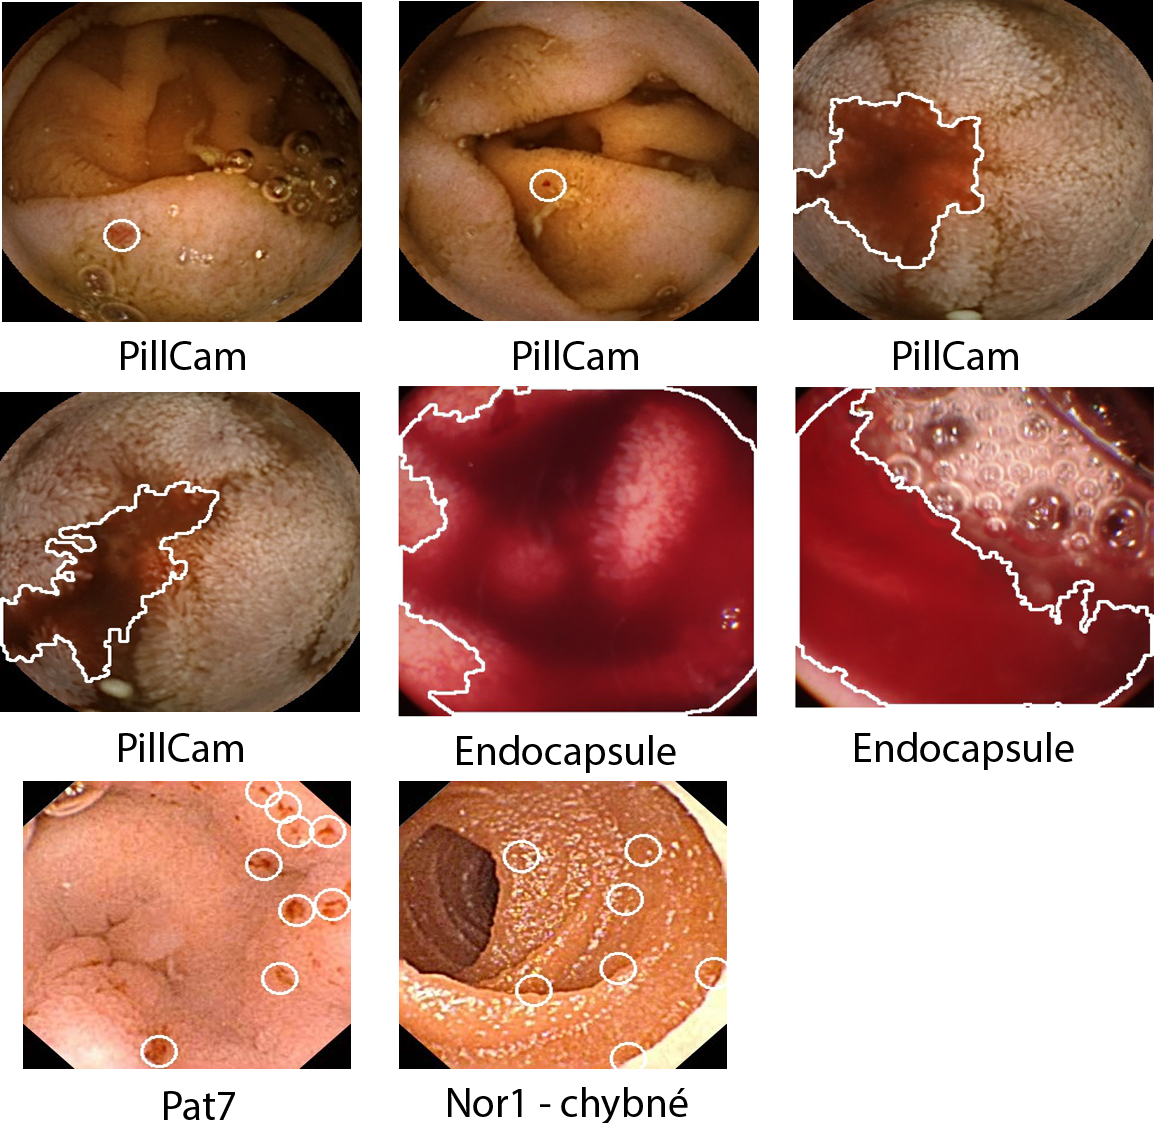
\includegraphics[scale=1.6]{result}
	\centering
	\caption{Ukázka vybraných výsledků \label{fig:vysledy}}
\end{figure}

\section{Zhodnocení testování}
Testování algoritmů probíhalo ve dvou etapách. V první etapě se algoritmy vyvíjeli a testovali na prvním vzorku dat. Kde se dle tabulky \ref{tab:vyslekdy_1} dosáhlo uspokojivých výsledků.

V druhé etapě byl obdržen druhý vzorek dat z reálných pacientů. Po aplikaci konfigurace z prvního vzorku a spuštění testů nad druhým došlo k téměř absolutnímu neúspěchu. Aplikace nebyla schopna detekovat ani výrazné krvácení. Bylo zapotřebí vytvořit konfiguraci, zejména na filtr dle barev, pro každý vzorek zvlášť. Stejné chování je zaznamenáno i mezi odlišnými výrobci kamer v druhém vzorku, každá kamera má odlišné barevné spektrum, které dokáže snímat a tak není možné použít univerzální řešení pro všechno. Výsledky testování druhého vzorku jsou vidět v tabulce \ref{tab:vyslekdy_2}.

Při testování jinak nedošlo ke změnám algoritmů či programu. Vše fungovalo, tak jak bylo očekáváno. Pouze se vytvořili nové konfigurace pro algoritmy. Porovnání nové metody o proti metodám zmíněných ve vědeckých článcích nebylo možné, protože není k dispozici stejný datový vzorek. V následující kapitole budou detailněji rozebrány a zhodnoceny samotné výsledky.